\documentclass[11pt,a4paper]{article}
\usepackage[T1]{fontenc}
\usepackage[utf8]{inputenc}
\usepackage{lmodern}
\usepackage[scaled=0.95]{helvet}
\renewcommand{\familydefault}{\sfdefault}
\usepackage[left=18mm,right=18mm,top=16mm,bottom=18mm]{geometry}
\usepackage[table]{xcolor}
\usepackage{graphicx,booktabs,tabularx,array,enumitem,titlesec,needspace,microtype}
\usepackage[most]{tcolorbox}
\usepackage{tikz}
\usetikzlibrary{positioning,arrows.meta}
\usepackage{fancyhdr}
\usepackage[hidelinks]{hyperref}

\definecolor{navy}{HTML}{01093D}
\definecolor{teal}{HTML}{08706D}
\definecolor{mint}{HTML}{E3F6F3}
\definecolor{soft}{HTML}{F3F6F7}
\definecolor{body}{HTML}{2B3245}
\definecolor{muted}{HTML}{5A6378}
\definecolor{amber}{HTML}{A65D00}
\definecolor{cream}{HTML}{FFF4E0}
\AtBeginDocument{\color{body}}
\setlength{\parindent}{0pt}
\setlength{\parskip}{5pt}
\linespread{1.04}
\setlength{\emergencystretch}{2em}
\renewcommand{\arraystretch}{1.25}
\setlist{leftmargin=1.3em,itemsep=3pt,topsep=3pt,parsep=0pt}
\titleformat{\section}{\LARGE\bfseries\color{navy}}{\color{teal}\thesection}{0.5em}{}
\titlespacing*{\section}{0pt}{5pt}{10pt}
\titleformat{\subsection}{\large\bfseries\color{navy}}{}{0em}{}
\titlespacing*{\subsection}{0pt}{10pt}{4pt}
\pagestyle{fancy}
\fancyhf{}
\renewcommand{\headrulewidth}{0pt}
\fancyfoot[L]{\footnotesize\color{muted}TendOlive \textperiodcentered\ Team preparation}
\fancyfoot[R]{\footnotesize\color{muted}\thepage}
\newtcolorbox{say}[1]{enhanced,colback=mint,colframe=teal,boxrule=0pt,leftrule=3pt,
  sharp corners,left=9pt,right=9pt,top=7pt,bottom=7pt,
  before upper={\textbf{\color{teal}#1}\par\smallskip}}
\newtcolorbox{note}[1]{enhanced,colback=cream,colframe=amber,boxrule=0pt,leftrule=3pt,
  sharp corners,left=9pt,right=9pt,top=7pt,bottom=7pt,
  before upper={\textbf{\color{amber}#1}\par\smallskip}}
\newcommand{\qa}[2]{\needspace{5\baselineskip}\textbf{\color{navy}#1}\par\nopagebreak
  #2\par\vspace{6pt}}
\newcommand{\smallref}[1]{{\footnotesize\color{muted}#1}}
\newcolumntype{Y}{>{\raggedright\arraybackslash}X}
\hypersetup{pdftitle={RAG: the jury brief},pdfsubject={TendOlive jury preparation}}

\begin{document}
\begin{minipage}[c]{0.66\textwidth}
{\fontsize{25}{28}\selectfont\bfseries\color{navy}RAG: the jury brief}
\end{minipage}\hfill
\begin{minipage}[c]{0.27\textwidth}\raggedleft

\includegraphics[width=\linewidth]{../brand/tendolive-logo.png}
\end{minipage}
\vspace{9pt}

\section{What the RAG contributes}
\begin{say}{The 30-second version}
A consulting firm must prove every claim in a bid: ``3 data engineers'', ``a PMP-certified project manager'', ``a health-sector reference''.
The proof is scattered across CVs and project records. Our RAG service reads each tender requirement, finds the
OliveSoft documents that could prove it, and decides: \textbf{covered, partial or missing}, with the \textbf{exact
line} that proves it. It never invents proof: when nothing proves a requirement, it says so and lists what to add.
\end{say}
\smallref{The quotes are copied from documents. The system can still select an unsuitable quote or make a wrong matching decision, so a person reviews the result.}

\subsection{Its place in the project}
RAG means \textbf{Retrieval-Augmented Generation}: retrieve useful information, then give it to a large language model (LLM) to help it write. In TendOlive, our service retrieves and checks the evidence; the proposal agents do the writing.

\begin{center}
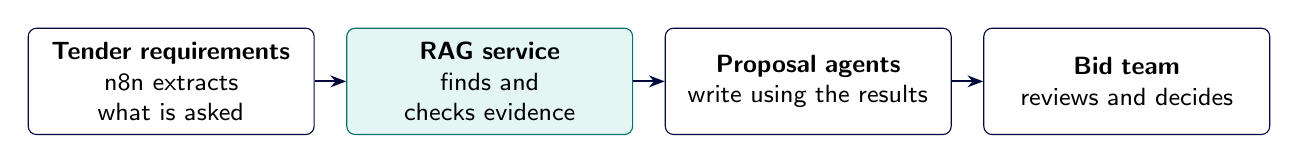
\begin{tikzpicture}[node distance=4mm,
  box/.style={draw=navy,rounded corners=3pt,align=center,text width=3.35cm,
    minimum height=1.35cm,inner sep=4pt,font=\small},
  arr/.style={-{Stealth[length=2mm]},line width=0.8pt,navy}]
\node[box] (a) {\textbf{Tender requirements}\\n8n extracts what is asked};
\node[box,right=of a,fill=mint,draw=teal] (b) {\textbf{RAG service}\\finds and checks evidence};
\node[box,right=of b] (c) {\textbf{Proposal agents}\\write using the results};
\node[box,right=of c] (d) {\textbf{Bid team}\\reviews and decides};
\draw[arr] (a)--(b); \draw[arr] (b)--(c); \draw[arr] (c)--(d);
\end{tikzpicture}
\end{center}

\textbf{Input:} lists of technical, team and experience requirements.\\
\textbf{Output:} a table showing each requirement, its status, a supporting document and quote, plus a proposed team and a gap report. A coverage score feeds the project's bid recommendation.

\subsection{A concrete example: ``2 data engineers''}
The service reads \textbf{role = data engineer} and \textbf{count = 2}. In the benchmark's 19 CVs, 8 profiles match that role. It marks the requirement \textbf{Covered}, proposes 2 people and cites a CV line such as:

\begin{quote}\small
``Data Engineer with 3+ years of experience designing and operating end-to-end data pipelines\ldots'' \hfill\textit{CV 13}
\end{quote}

\begin{tabularx}{\textwidth}{@{}>{\bfseries}p{2.1cm}Y@{}}
\toprule
Covered & Enough matching evidence: 2 data engineers requested, 8 found.\\
Partial & Some evidence, but a gap: 3 \emph{senior} data engineers requested, only 1 found.\\
Missing & No qualifying evidence found in the indexed documents.\\
\bottomrule
\end{tabularx}
\par\smallskip
\textbf{Missing means the documents do not prove it.} It does not establish that OliveSoft lacks the capability.

\newpage
\section{How it works}

\subsection{Before a tender: prepare the documents}
The knowledge base contains CVs and records about projects, technologies, tools and clients. Indexing prepares two useful views of this information:
\begin{itemize}
\item \textbf{A fact card for each document:} the skills, roles, certificates and experience levels that the rules extract. For CVs, certificates are read from the Certifications section.
\item \textbf{A searchable collection of text pieces:} documents are split into overlapping pieces called \emph{chunks}. An \emph{embedding model} converts each piece into numbers representing its meaning. ChromaDB stores these numbers for search. The original text is kept for quotations.
\end{itemize}
Adding a document updates this index; it does not retrain the AI models.

\subsection{For each requirement: four steps}
\begin{enumerate}[leftmargin=1.6em,itemsep=8pt]
\item \textbf{Read what is being requested.}\\
A French/English vocabulary and rules identify known skills, roles, certificates, counts and seniority. For example, ``3 senior data engineers'' becomes a role, a level and a required number of people.

\item \textbf{Search in two complementary ways.}\\
\textbf{BM25} searches by words, which helps with exact names such as Power BI or a certificate code. \textbf{E5} searches by meaning, which helps with different wording and languages. The two ranked lists are merged. This is \emph{hybrid search}.

\item \textbf{Assess whether the documents support the requirement.}\\
When the rules can interpret the requirement's constraints, they check the document facts and count the matches. When wording remains outside the vocabulary, a \textbf{reranker} reads the requirement and each of the top five candidate documents together and scores how well they match. It is an AI matching model, not the model that writes the proposal.

\item \textbf{Return the assessment and its evidence.}\\
The service assigns Covered, Partial or Missing and looks for a supporting quote. Weak evidence cannot by itself justify Covered. Team selection uses matching CVs; the gap report identifies what is still missing.
\end{enumerate}

\begin{say}{When the reranker helps: ``vector database''}
In the documented example, ``vector'' is outside the rule vocabulary, so the reranker assesses the search candidates. CV 12 contains:

\textit{``Integrated LangChain and Pinecone vector databases to power semantic search and Retrieval-Augmented Generation''.}

The service returns Covered. Here, search finds candidates and the reranker assesses them; for ``2 data engineers'', the decision depends on counting matching profiles.
\end{say}

\textbf{What the rules protect against:} mentioning project management does not establish PMP certification. The CV must list the requested certificate. A recognised alternative can be marked Partial for a person to check.

\newpage
\section{Why these choices, and what we tested}

\subsection{The choices to be able to explain}
\begin{tabularx}{\textwidth}{@{}>{\bfseries\raggedright\arraybackslash}p{4.0cm}Y@{}}
\toprule
Choice & Reason\\
\midrule
Keywords + meaning & Exact product names matter, but tenders and CVs can use different wording. Each search method helps with the other's misses.\\
Rules for explicit constraints & A similarity score alone does not check whether there are enough people or whether a certificate is actually listed.\\
Reranker for other wording & The vocabulary is limited. A model that reads the requirement and document together provides a fallback.\\
Quotes and gap reporting & The reviewer needs to inspect the evidence and see what is missing before making a bid claim.\\
Local retrieval and checking & The RAG service runs on CPU without a paid AI API. Proposal generation is a separate part with its own model configuration.\\
\bottomrule
\end{tabularx}

\subsection{How we evaluated it}
Expected answers were prepared from the documents and compared with the service's outputs. We compared search methods and decision methods on shared test cases, using separate benchmark indexes. We checked both \textbf{which documents were retrieved} and \textbf{whether the resulting assessments were correct}.

\begin{tabularx}{\textwidth}{@{}>{\raggedright\arraybackslash}p{3.5cm}>{\bfseries\raggedright\arraybackslash}p{2.7cm}Y@{}}
\toprule
Test & Result & What this tells us\\
\midrule
42 internal CV checks & 8 $\rightarrow$ 15 $\rightarrow$ 40 passed & Similarity threshold alone, reranker alone, then rules + reranker. The rules helped on these checks.\\
20 requirements from 6 BOAMP tenders & 16 correct statuses & A small test on additional tender wording. It is not a fully independent evaluation.\\
\bottomrule
\end{tabularx}
\par\smallskip
\smallref{BOAMP is a source of French public procurement notices. Figures come from saved evaluations; the main benchmark run is dated 30 October 2026.}

\begin{note}{What these results do not establish}
\begin{itemize}[leftmargin=1.2em,itemsep=4pt]
\item \textbf{40/42 is an internal development result.} The checks do not establish performance on all future tenders or prove every quoted constraint.
\item \textbf{16/20 is not an untouched test.} AI drafted the expected answers and a second AI reviewed them; some vocabulary fixes used this set. A human review and a fresh test set are needed for stronger evidence.
\item \textbf{A correct status can come with an unsuitable citation.} On the additional tenders, the lead document matched a reference document on only 3 of 10 comparable rows. This is agreement with the reference, not a complete judgment of every alternative document.
\end{itemize}
\end{note}

\textbf{A concrete failure to remember:} ``Blockchain smart contracts'' was marked Partial when the expected answer was Missing. Generic words in unrelated CVs can still create a false match.

\newpage
\section{Answers for the jury}
\smallref{Start with the short answer. Add an example or a result if the jury asks for more.}
\vspace{7pt}

\qa{What did you build in the RAG part?}{A service that takes tender requirements, searches the company's documents, checks what those documents support, and returns statuses, evidence, a proposed team and missing information. Its results feed the web app and the proposal workflow.}

\qa{Where is the generation in your RAG?}{The proposal agents use an LLM to write from the retrieved results. Our RAG service handles retrieval and assessment. It uses embedding and reranking models, but no generative LLM to make the coverage decisions.}

\qa{Why not put all the CVs into an LLM prompt?}{We wanted explicit checks for counts and certifications, traceable quotes and results we can test consistently. We did not benchmark this system against a full LLM-prompting approach, so we cannot claim it outperforms that alternative.}

\qa{Why do you need both rules and AI?}{The rules check known constraints, such as ``two people'' or ``PMP certified''. The AI search and reranker help with varied wording. The vocabulary needs maintenance, and the AI fallback can still make mistakes.}

\qa{Can it invent or misrepresent evidence?}{It copies quotations from the documents rather than generating them. However, it can select an irrelevant document or interpret a match incorrectly. We check quote relevance, flag gaps and keep human review in the process.}

\qa{Does a high fit score mean we will win the tender?}{No. It measures documented coverage of the requirements. Code uses the matrix to suggest a bid action, but pricing, availability and the final decision still need human judgment.}

\qa{How did you test it, and how strong are the results?}{We compared outputs with expected answers from the documents. The final system passed 40 of 42 internal CV checks and got 16 of 20 statuses right on additional BOAMP requirements. Both are small, development-influenced sets; they are not a guarantee of performance on new tenders.}

\qa{Do CVs leave the machine?}{Retrieval and matching run locally. The proposal-writing model can receive selected evidence; the documented default uses Groq. Privacy therefore depends on the full pipeline configuration, not only the RAG service.}

\qa{What would you improve next?}{Evidence selection on new tenders, ambiguous wording and independent evaluation. We would have a person check the labels, then test on fresh requirements that were not used to adjust the rules.}

\newpage
\section*{Technical reference \textnormal{\large(optional)}}
\smallref{Use this page for follow-up questions. The main explanation is on pages 1--4.}
\vspace{7pt}

\qa{Which models and storage do you use?}{Multilingual E5-small creates the embeddings; ChromaDB stores them locally. The reranker is a multilingual MiniLM cross-encoder. The service uses FastAPI and runs in Docker on CPU.}

\qa{How does French support work?}{A French/English vocabulary supplies aliases for keyword search, and E5 supports search across languages. The pipeline generally sends short English requirements. Difficult French wording can still be missed.}

\qa{When exactly do the rules decide?}{The parser must identify at least one known constraint and leave no unexplained wording after recognised filler and context words are handled. Otherwise the reranker assesses the line. Known certificate requirements still constrain which CVs can qualify.}

\qa{How are the two search lists merged?}{Reciprocal Rank Fusion (RRF) combines document positions in the two lists. A document ranked well by either search can rise in the combined list; the raw keyword and similarity scores do not need the same scale.}

\qa{How is the team selected?}{The service searches for a small set of qualifying CVs covering the requested headcounts. One person can satisfy several requirement lines. It uses exhaustive search up to a limit, then a greedy fallback; near matches are not staffed. This is a document-based proposal, not an availability check.}

\qa{Why did you use direct benchmarks rather than RAGAS?}{Our main outputs are statuses, counts and selected documents, so we compared them directly with expected answers and used retrieval metrics. Assessing whether the generated proposal stays faithful to the evidence would be a separate evaluation.}

\subsection{Useful implementation details}
{\small
\begin{tabularx}{\textwidth}{@{}>{\bfseries\raggedright\arraybackslash}p{3.4cm}Y@{}}
\toprule
Embedding model & \texttt{intfloat/multilingual-e5-small}\\
Reranker model & \texttt{cross-encoder/mmarco-mMiniLMv2-L12-H384-v1}\\
Chunks & 200 words, with 50 words of overlap\\
Search and reranking & 50 dense-search chunks; up to 5 candidate documents reranked\\
Returned evidence & Normally up to 3 proof documents per line; headcount requirements can need more\\
Main integration & \texttt{POST /retrieve/tender}; results appear in the web app\\
Knowledge base & 19 CVs, 37 projects, 5 technology stacks, 4 tools, 25 client records in the reference Company corpus; Demo has a separate index\\
\bottomrule
\end{tabularx}}

\subsection{Where to check the details}
\smallref{In the TendOlive repository: \texttt{docs/rag-service.md} explains matching; \texttt{docs/rag-benchmark.md} explains evaluation. Saved results are in \texttt{services/rag/benchmark/results.md} and \texttt{services/rag/benchmark/independent/results.md}. Configuration is in \texttt{services/rag/rag/config.py}.}

\end{document}
